% !TeX TXS-program:compile = txs:///arara
% arara: lualatex: {shell: no, synctex: yes, interaction: batchmode}
% arara: pythontex: {rerun: modified} if found('pytxcode', 'PYTHONTEX#py')
% arara: lualatex: {shell: no, synctex: yes, interaction: batchmode} if found('pytxcode', 'PYTHONTEX#py')
% arara: lualatex: {shell: no, synctex: yes, interaction: batchmode} if found('log', '(undefined references|Please rerun|Rerun to get)')

\documentclass[a4paper,11pt]{article}
\usepackage[revgoku]{cp-base}
\graphicspath{{./graphics/}}
%variables
\donnees[classe={1\up{ère} 2M2},matiere={[SPÉ.MATHS]},mois=Juin,annee=2022,typedoc=CHAP,numdoc=12]

%formatage
\author{Pierquet}
\title{\nomfichier}
\hypersetup{pdfauthor={Pierquet},pdftitle={\nomfichier},allbordercolors=white,pdfborder=0 0 0,pdfstartview=FitH}
%fancy
\lhead{\entete{\matiere}}
\chead{\entete{\lycee}}
\rhead{\entete{\classe{} - \mois{} \annee}}
\lfoot{\pied{\matiere}}
\cfoot{\logolycee{}}
\rfoot{\pied{\numeropagetot}}
%divers
\usepackage{epsdice}

\begin{document}

\pagestyle{fancy}

\part{CH12 - Variables aléatoires - Exercices (Correction)}

\medskip

\exonum{0}

\begin{enumerate}
	\item La loi de probabilité de $X$ est :
	\begin{center}
		\begin{tabularx}{60mm}{|Y|Y|Y|Y|}
			\hline
			$x_i$ & $0$ & $3$ & $10$ \\ \hline
			$p_i$ & $\nicefrac{16}{32}$ & $\nicefrac{4}{32}$ & $\nicefrac{12}{32}$ \\ \hline
		\end{tabularx}
	\end{center}
	En effet, il y a 12 figures ($X=10$), 4 cartes dix ($X=3$) donc 16 cartes restantes ($X=0$).
	\item La loi de probabilité de $Y$ est :
	\begin{center}
		\begin{tabularx}{60mm}{|Y|Y|Y|Y|Y|Y|}
			\hline
			$x_i$ & $-37$ & $9$ & $13$ & $25$ & $50$ \\ \hline
			$p_i$ & $\nicefrac{16}{32}$ & $\nicefrac{10}{32}$ & $\nicefrac{2}{32}$ & $\nicefrac{3}{32}$ & $\nicefrac{1}{32}$ \\ \hline
		\end{tabularx}
	\end{center}
	En effet, il y 1 as de trèfle ($X=50$), 3 autres as ($X=25$), le roi et la dame de pique ($X=13$), 10 autres figures ($X=9$) et 16 autres cartes ($X=-37$).
\end{enumerate} 

\medskip

\exonum{1}

\begin{enumerate}
	\item On a :
	\begin{itemize}
		\item $\esp{X}=-5 \times 0,3 + 0 \times 0,4 + 7 \times 0,3 = 0,6$ ;
		\item $\var{X}=(-5)^2 \times 0,3 + 0^2 \times 0,4 + 7^2 \times 0,3 - 0,6^2 = 21,84$ et donc $\sigma(X)=\sqrt{21,84} \approx 4,67$.
	\end{itemize}
	\item On a :
	\begin{itemize}
		\item $\esp{X}=-4 \times 0,2 + (-3) \times 0,3 + 2 \times 0,4 + 5 \times 0,1 = -0,4$ ;
		\item $\var{X}=(-4)^2 \times 0,2 + (-3)^2 \times 0,3 + 2^2 \times 0,4 + 5^2 \times 0,1 - (-0,4)^2 = 9,84$ et donc $\sigma(X)=\sqrt{9,84} \approx 3,14$.
	\end{itemize}
\end{enumerate}

\medskip

\exonum{1}

\begin{center}
	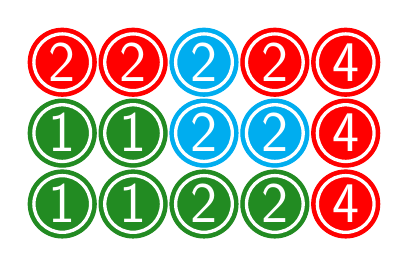
\begin{tikzpicture}[scale=0.9]
		\foreach \centre/\couleur/\numero in {%
			(0,0)/ForestGreen/1,(1,0)/ForestGreen/1,(2,0)/ForestGreen/2,(3,0)/ForestGreen/2,(4,0)/red/4,%
			(0,1)/ForestGreen/1,(1,1)/ForestGreen/1,(2,1)/cyan/2,(3,1)/cyan/2,(4,1)/red/4,%
			(0,2)/red/2,(1,2)/red/2,(2,2)/cyan/2,(3,2)/red/2,(4,2)/red/4}{%
				\filldraw[\couleur] \centre circle[radius=0.48] node[white] {\huge \sf \numero} ;
				\draw[very thick,white] \centre circle[radius=0.4] ;}
	\end{tikzpicture}
\end{center}
%
\begin{enumerate}
	\item La loi de probabilité de $X$ est :
	
	\begin{center}
		\SetTblrDefault{rowsep=1pt,colsep=1pt}
		\begin{tblr}{hlines={0.45pt},vlines={0.45pt},columns={15mm,c}}
			$x_i$ & $1$ & $2$ & $4$ \\
			$p_i$ & $\nicefrac{4}{15}$ & $\nicefrac{8}{15}$ & $\nicefrac{3}{15}$ \\
		\end{tblr}
	\end{center}
	En effet, il y quatre boules \textcircled{\sf 1} ($X=1$), huit boules \textcircled{\sf 2} ($X=2$) et trois boules \textcircled{\sf 4} ($X=4$).
	\item  La loi de probabilité de $Y$ est :
	\begin{center}
		\SetTblrDefault{rowsep=1pt,colsep=1pt}
		\begin{tblr}{hlines={0.45pt},vlines={0.45pt},columns={15mm,c}}
			$y_i$ & $1$ & $2$ & $4$ \\
			$p_i$ & $\nicefrac{3}{15}$ & $\nicefrac{10}{15}$ & $\nicefrac{2}{15}$ \\
		\end{tblr}
	\end{center}
	En effet, il y a :
	\begin{itemize}
		\item quatre boules \textcircled{\sf 1} vertes, trois boules \textcircled{\sf 4} rouges et trois boules \textcircled{\sf 2} bleues ($Y=2$) ;
		\item trois boules \textcircled{\sf 2} rouges ($Y=1$) ;
		\item deux boules \textcircled{\sf 2} vertes ($Y=4$).
	\end{itemize}
\end{enumerate}

\medskip

\exonum{2}

\begin{enumerate}
	\item On peut proposer le tableau suivant :
	\begin{center}
		\SetTblrDefault{rowsep=0pt,colsep=0pt}
		{\Large \begin{tblr}{columns={7mm,c},rows={7mm},vline{1}={2-7}{solid},vline{2-8}={solid},hline{1}={2-7}{solid},hline{2-8}={solid}}
			 & \epsdice{1} & \epsdice{2} & \epsdice{3} & \epsdice{4} & \epsdice{5} & \epsdice{6} \\
			\epsdice[black]{1} & 2 & 3 & 4 & 5 & 6 & 7 \\
			\epsdice[black]{2} & 3 & 4 & 5 & 6 & 7 & 8 \\
			\epsdice[black]{3} & 4 & 5 & 6 & 7 & 8 & 9 \\
			\epsdice[black]{4} & 5 & 6 & 7 & 8 & 9 & 10 \\
			\epsdice[black]{5} & 6 & 7 & 8 & 9 & 10 & 11 \\
			\epsdice[black]{6} & 7 & 8 & 9 & 10 & 11 & 12 \\
		\end{tblr}}
	\end{center}
	\item La loi de probabilité de $S$ est :
	\begin{center}
		\SetTblrDefault{rowsep=1pt,colsep=1pt}
		\begin{tblr}{hlines={0.45pt},vlines={0.45pt},hline{1-3}={1-{12}}{solid},columns={9mm,c}}
			$s_i$ & $2$ & $3$ & $4$ & $5$ & $6$ & $7$ & $8$ & $9$ & $10$ & $11$ & $12$ \\
			$p_i$ & $\nicefrac{1}{36}$ & $\nicefrac{2}{36}$ & $\nicefrac{3}{36}$ & $\nicefrac{4}{36}$ & $\nicefrac{5}{36}$ & $\nicefrac{6}{36}$ & $\nicefrac{5}{36}$ & $\nicefrac{4}{36}$ & $\nicefrac{3}{36}$ & $\nicefrac{2}{36}$ & $\nicefrac{1}{36}$ \\
		\end{tblr}
	\end{center}
	\item On a $\esp{S}=2 \times \dfrac{1}{36} + 3 \times \dfrac{2}{36} + \ldots + 11 \times \dfrac{2}{36} + 12 \times \dfrac{1}{36} = 7$.
	
	Ainsi en lançant deux dés et en additionnant les faces, on obtient en moyenne 7.
\end{enumerate}

\medskip

\exonum{2}

\begin{enumerate}
	\item Le tableau complété est :
	\begin{center}
		\SetTblrDefault{rowsep=3pt,colsep=3pt}
		\begin{tblr}{colspec={Q[22mm,c]Q[22mm,c]Q[22mm,c]Q[22mm,c]Q[22mm,c]},%
				     rowspec={Q[m]Q[m]Q[m]Q[m]},%
			     	 vline{1}={2-5}{solid},vline{2-6}={solid},hline{1}={2-6}{solid},hline{2-5}={solid}}
			& \textbf{Weekend \\ uniquement} & \textbf{Weekend \\ et semaine} & \textbf{En salle} & \textbf{Total} \\
			\textbf{Fitness} & 20 & 10 & 70 & 100 \\
			\textbf{Pas fitness} & 130 & 190 & 30 & 350 \\
			\textbf{Total} & 150 & 200 & 100 & 450 \\
		\end{tblr}
	\end{center}
	\item 
	\begin{enumerate}
		\item Les valeurs prises par $X$ sont :
		\begin{itemize}
			\item 400 : en salle sans fitness ;
			\item 430 : en salle avec fitness ;
			\item 450 : w-end sans fitness ;
			\item 480 : w-end avec fitness ;
			\item 505 : w-end semaine sans fitness ;
			\item 535 : w-end semaine avec fitness.
		\end{itemize}
		\item La loi de probabilité de $X$ est :
		\begin{center}
			\SetTblrDefault{rowsep=1pt,colsep=1pt}
			\begin{tblr}{hlines={0.45pt},vlines={0.45pt},columns={15mm,c}}
				$x_i$ & $400$ & $430$ & $450$ & $480$ & $505$ & $535$ \\
				$p_i$ & $\nicefrac{30}{450}$ & $\nicefrac{70}{450}$ & $\nicefrac{130}{450}$ & $\nicefrac{20}{450}$ & $\nicefrac{190}{450}$ & $\nicefrac{10}{450}$ \\
			\end{tblr}
		\end{center}
	\end{enumerate}
	\item On a $\esp{X}=400 \times \dfrac{30}{450}+\ldots+535 \times \dfrac{10}{450}=470$.
	
	De ce fait, le prix moyen à l'année est de 470\,€.
\end{enumerate}

\pagebreak

\exonum{2}

\begin{enumerate}
	\item L'arbre de probabilités est : 
	%	
	\begin{center}
		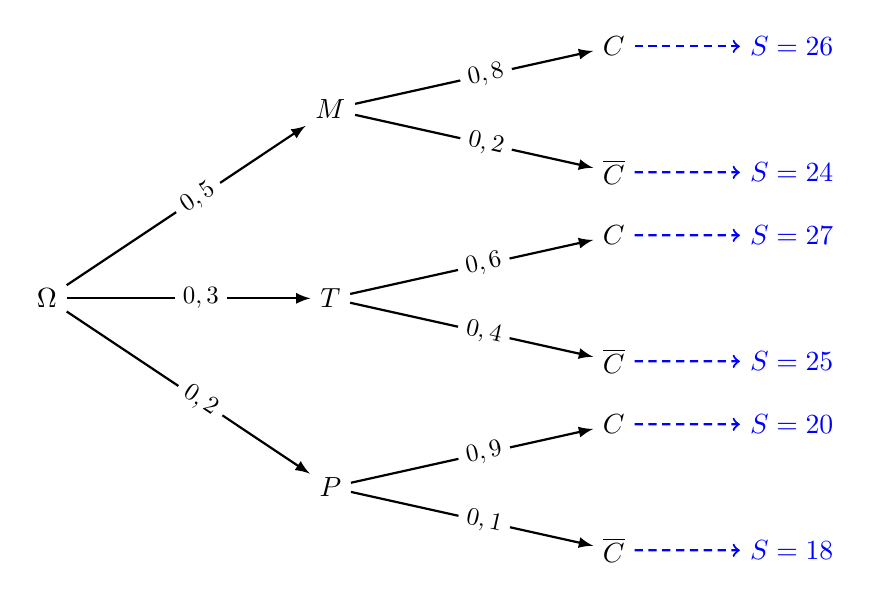
\begin{tikzpicture}[scale=0.8]
			\tikzstyle{fleche}=[->,>=latex,thick]
			\tikzstyle{noeud}=[]
			\tikzstyle{feuille}=[]
			\tikzstyle{etiquette}=[pos=0.55,sloped,fill=white,scale=0.9]
			\tikzstyle{vide}=[]
			
			\def\DistanceInterNiveaux{3}
			\def\DistanceInterFeuilles{1}
			
			\def\NiveauA{(0)*\DistanceInterNiveaux}
			\def\NiveauB{(1.5)*\DistanceInterNiveaux}
			\def\NiveauC{(3)*\DistanceInterNiveaux}
			\def\InterFeuilles{(-1)*\DistanceInterFeuilles}
			
			\node[noeud] (R) at ({\NiveauA},{(4)*\InterFeuilles}) {$\Omega$};
			\node[noeud] (Ra) at ({\NiveauB},{(1)*\InterFeuilles}) {$M$};
			\node[feuille] (Raa) at ({\NiveauC},{(0)*\InterFeuilles}) {$C$};
			\node[feuille] (Rac) at ({\NiveauC},{(2)*\InterFeuilles}) {$\overline{C}$};
			\node[noeud] (Rb) at ({\NiveauB},{(4)*\InterFeuilles}) {$T$};
			\node[feuille] (Rba) at ({\NiveauC},{(3)*\InterFeuilles}) {$C$};
			\node[feuille] (Rbc) at ({\NiveauC},{(5)*\InterFeuilles}) {$\overline{C}$};
			\node[noeud] (Rc) at ({\NiveauB},{(7)*\InterFeuilles}) {$P$};
			\node[feuille] (Rca) at ({\NiveauC},{(6)*\InterFeuilles}) {$C$};
			\node[feuille] (Rcc) at ({\NiveauC},{(8)*\InterFeuilles}) {$\overline{C}$};
			
			\draw[fleche] (R)--(Ra) node[etiquette] {$0,5$};
			\draw[fleche] (Ra)--(Raa) node[etiquette] {$0,8$};
			\draw[fleche] (Ra)--(Rac) node[etiquette] {$0,2$};
			\draw[fleche] (R)--(Rb) node[etiquette] {$0,3$};
			\draw[fleche] (Rb)--(Rba) node[etiquette] {$0,6$};
			\draw[fleche] (Rb)--(Rbc) node[etiquette] {$0,4$};
			\draw[fleche] (R)--(Rc) node[etiquette] {$0,2$};
			\draw[fleche] (Rc)--(Rca) node[etiquette] {$0,9$};
			\draw[fleche] (Rc)--(Rcc) node[etiquette] {$0,1$};
			
			\draw[blue,->,densely dashed,thick] (Raa) --++ (2,0) node[right] {$S=26$} ;
			\draw[blue,->,densely dashed,thick] (Rac) --++ (2,0) node[right] {$S=24$} ;
			\draw[blue,->,densely dashed,thick] (Rba) --++ (2,0) node[right] {$S=27$} ;
			\draw[blue,->,densely dashed,thick] (Rbc) --++ (2,0) node[right] {$S=25$} ;
			\draw[blue,->,densely dashed,thick] (Rca) --++ (2,0) node[right] {$S=20$} ;
			\draw[blue,->,densely dashed,thick] (Rcc) --++ (2,0) node[right] {$S=18$} ;
		\end{tikzpicture}
	\end{center}
	\item  
	\begin{enumerate}
		\item $M \cap C$ représente l'évènement \og le client a pris un macaron \textbf{et} un café \fg.
		
		Et on a $p(M \cap C) = p(M) \times p_M(C) = 0,5 \times 0,8 = 0,4$. 
		\item D'après la formule des probabilités totales, on a $p(C) = p(M \cap C) + p(T \cap C) + p(P \cap C)$.
		
		Et donc $p(C) = 0,4 + 0,3 \times 0,6 + 0,2 \times 0,9 =  0,4 + 0,18 + 0,18 = 0,76$.
	\end{enumerate} 
	\item Il faut trouver $p_C (M) = \dfrac{p(C \cap M)}{p(C)} = \dfrac{0,4}{0,76} \approx 0,53$ à 0,01 près.
	\item
	\begin{enumerate}
		\item  On a :
		
		\tabula{}$\bullet~~P + M + C$ : 18 + 6 + 2 = 26~\euro ;
		
		\tabula{}$\bullet~~P + M$ : 18 + 6 = 24~\euro ;
		
		\tabula{}$\bullet~~P + T + C$ : 18 + 7 + 2 = 27~\euro ;
		
		\tabula{}$\bullet~~P + T$ : 18 + 7 = 25~\euro ;
		
		\tabula{}$\bullet~~P + C$  : 18 + 2 = 20~\euro ;
		
		\tabula{}$\bullet~~P$ : 18~\euro
		\item Le tableau complété est :
		
		\begin{center}
			\SetTblrDefault{rowsep=3pt,colsep=3pt}
			\begin{tblr}{hlines={0.45pt},vlines={0.45pt},width=10.5cm,%
					colspec={X[1.75,c]X[c]X[c]X[c]X[c]X[c]X[c]}}
				Sommes $s_{i}$& 18 &20 &24 &25&26&27\\ 
				$p\left(s_{i}\right)$&$0,02$&$0,18$	&$0,1$	&$0,12$	&$0,4$	&$0,18$\\
			\end{tblr}
		\end{center}
		\item On a $18 \times 0,02 + 20 \times0,18 + 24 \times0,1 + 25 \times0,12 + 26 \times 0,4 + 27 \times 0,18 = 24,62$~(\euro).
		
		Sur un grand nombre de repas la recette par client s'élève à 24,62~\euro. 
	\end{enumerate}
\end{enumerate}

\end{document}